%%=============================================================================
%% Methodologie
%%=============================================================================
\chapter{Methodologie}
\label{ch:methodologie}

%% TODO: Hoe ben je te werk gegaan? Verdeel je onderzoek in grote fasen, en
%% licht in elke fase toe welke stappen je gevolgd hebt. Verantwoord waarom je
%% op deze manier te werk gegaan bent. Je moet kunnen aantonen dat je de best
%% mogelijke manier toegepast hebt om een antwoord te vinden op de
%% onderzoeksvraag.

In dit hoofdstuk zal er besproken worden hoe er een antwoord zal gevonden worden op de onderzoeksvragen. 

\section{Verzamelen van gegevens}
\label{sec:verzamelen}

Om antwoord te krijgen op welke functionaliteiten en functies gebruikers zoeken in gezondheidsapplicaties moeten er natuurlijk gegevens verzameld worden. Daarom is er binnen dit onderzoek gekozen om een vragenlijst op te stellen. Deze vragenlijst wordt verspreid via sociale media, er zullen expliciet groepen gezocht worden waarin mensen gebruik maken van dergelijke applicaties of programma’s. 

bestaan tegenwoordig heel veel facebook groepen over gezondheid, een groot voordeel van deze groepen is dat er een actieve community is. Er is dan ook gekozen voor facebook groepen waar er veel reactie op berichten komt. Er zal ook geprobeerd worden om de vragenlijst op Facebookpagina’s van fitnesscentra te krijgen.

\section{Gebruikte technologie voor de vragenlijst}
\label{sec:gebruikte-technologie}

Om de vragenlijst aangenamer te maken tijdens het invullen, is er voor dit onderzoek zelf een kleine PHP-applicatie geschreven. De tool is geschreven via een bootstrap-framework met alle nodige functionaliteiten voor dit onderzoek en is ook ‘mobile responsive’ zodat gebruikers van mobiele toestellen makkelijk kunnen deelnemen aan het onderzoek. De belangrijkste functie is natuurlijk het wegschrijven van de ingevulde gegevens. Er is gekozen om alle data naar een CSV-bestand weg te schrijven. Een CSV-bestand is makkelijk in te lezen in RStudio om de gegevens te analyseren.

De code van de tool kan teruggevonden worden in de bijlage. De applicatie zelf is terug te vinden op: https://vragenlijst.dndesign.be/ .

\section{Het opstellen van de vragenlijst}
\label{sec:opstellen-vragenlijst}

De vragen die gekozen zijn om de vragenlijst op te stellen komen hoofdzakelijk uit de literatuurstudie in het voorgaande hoofdstuk. Er zijn een paar vragen die overgenomen zijn maar er zijn ook een aantal nieuwe bijgekomen door het kritisch lezen van de artikelen uit de literatuurstudie. Anderzijds zijn er ook een aantal vragen terug te vinden uit persoonlijke ervaring met gezondheidsapplicaties. 

Het doel van de van de vragenlijst was dat deelnemers niet zomaar zouden door klikken op het einde, daarom is ervoor gekozen om de enquête kort te houden. Zonder al te lange vragen of antwoorden waar deelnemers lang moesten over nadenken. 
Een andere troef van de vragenlijst is dat deze volledig anoniem wordt ingevuld, op geen enkel moment wordt de naam of andere contactgegevens van de deelnemer gevraagd. Hierdoor zal er een groter deel van de mensen makkelijker willen deelnemen aan het onderzoek.

De vragenlijst is opgebouwd uit 3 delen: 

\subsection{Persoonsgegevens}

Zoals hierboven al is vermeld, worden er geen contactgegevens gevraagd. De persoonsgegevens zullen belangrijke parameters zijn in het vervolg van dit onderzoek. 

De persoonsgegevens zijn een makkelijke indicator om verschillende groepen te bekijken op basis van geslacht en leeftijd. 

\begin{table}[h!]
\begin{center}
\begin{tabular}{ |p{3cm}|p{7cm}| }
 \hline
 Parameter 1:   & Geslacht  \\
 \hline
Parameter 2: &   Leeftijd   \\
 \hline
 Parameter 3: &   Aantal keren sport per week   \\
 \hline
 Parameter 4: &  Besturingssysteem van smartphone   \\
 \hline
   Parameter 5: & Heeft u al een mobile coaching applicatie gebruikt? \\
 \hline
\end{tabular}
\end{center}
\caption{Persoonsgegevens}
\label{table:1}
\end{table}
\newpage


\subsection{App Requirements}

In dit onderdeel zal een antwoord gezocht worden op wat gebruikers graag in de applicatie willen zien. De vragen zijn zowel functioneel als niet-functioneel gericht. Dit deel is hoofdzakelijk bedoeld om te achterhalen wat gebruikers zoeken en verwachten van mobiele coaching applicaties. 

Er is gekozen om gesloten vragen te stellen omdat er redelijk wat input verwacht wordt, de gesloten vragen zijn makkelijker om te analyseren. En in de tweede fase van ons onderzoek hebben we de gesloten antwoorden nodig als trainingsdata voor Machine Learning. Dit zou niet mogelijk geweest zijn indien er gebruik gemaakt werd van open vragen.

\begin{table}[h!]
\begin{center}
\begin{tabular}{ |p{11cm}|p{3cm}| }
 \hline
 \textbf{Vraag}   &  \textbf{Type} \\
 \hline
Vindt u het belangrijk om de applicatie met een smartwatch of dergelijke te connecteren? &   Functioneel   \\
 \hline
 Bent u bereid te betalen voor een applicatie? &  Niet-Functioneel   \\
 \hline
 Hoe belangrijk vindt u het uitzicht en gebruiksgemak van een applicatie? &  Niet-Functioneel  \\
 \hline
   Is het belangrijk dat u de applicatie kan koppelen aan social media? & Functioneel \\
 \hline
    Vindt u het belangrijk dat een applicatie gebruik maakt van uw geolocatie (GPS)? bv. om uw traject te zien? & Functioneel \\
 \hline
    Ik vind extra uitleg of filmpjes bij oefeningen... & Functioneel \\
 \hline
  Wat is uw hoofddoel bij het gebruik van een Mobile Coaching applicatie? & Niet-Functioneel \\
 \hline
\end{tabular}
\end{center}
\caption{App requirements}
\label{table:1}
\end{table}

\subsection{Type gebruiker bepalen}

In het laatste deel van de vragenlijst heeft de deelnemer 3 keuzes om uit te kiezen. De deelnemer dient het antwoord te kiezen die het best bij zijn gebruikersdoel van een mobile coaching applicaties past. Er is keuze uit: Enkel voedingsschema’s, enkel trainingsschema’s of coaching applicaties. Dit zal een andere bepaalde factor zijn voor het tweede deel van het onderzoek waarbij we Machine Learning zullen gebruiken om aan de hand van app requirements of het gebruikersdoel een type gebruiker proberen te voorspellen. 

\section{Bestaande applicaties vergelijken}
\label{sec:applicaties-vergelijken}

Om een antwoord te formuleren op de vraag ‘welke applicaties zijn er op de markt en voldoen deze applicaties aan de kritische punten?’ zullen de applicaties die beschreven zijn in de literatuurstudie per categorie onderling met elkaar vergeleken worden. Vervolgens zal de beste applicatie volgens de kritische punten van dit onderzoek bepaald worden. 

\newpage
\subsection{Kritische punten}

De kritische punten binnen dit onderzoek zullen uit 2 delen bestaan. Enerzijds zullen er kritische punten uit de literatuurstudie komen. De vragen die gesteld zullen worden zijn: Wie heeft de applicatie ontwikkeld? Heeft de maker voldoende ervaring en kennis binnen de gezondheidssector om dergelijke applicaties te publiceren? Zijn de algemene functies beperkt of uitgebreid? Hoe ziet de user interface er uit? Zijn bestaande gebruikers tevreden over de applicatie?

Anderzijds zal er binnen dit onderzoek ook een vragenlijst afgenomen worden. Nadat de gegevens van de vragenlijst geannalyseerd zijn, zal er gekeken worden naar zaken die gebruikers zeker in de applicatie willen. 

\section{Verband tussen gebruikersdoel en type applicatie bepalen }
\label{sec:machine-learning}

\subsection{Artificiële intelligentie of Machine Learning}

Eerst en vooral is Artificiële inteligentie een overkoepelend begrip. Het is een technologie waarbij computers gebruikt worden om het brein van mensen na te bootsen. Computers voeren taken uit op basis van een algoritme op een intelligente manier. 

Machine Learning is een onderverdeling van Artificiële intelligentie. In dit geval ontvangt de computer een bepaalde hoeveelheid data. De computer zal de data gebruiken om zichzelf te trainen. De training op zich gebeurt door de neurale netwerken. Het neurale netwerk probeert patronen te herkennen die hij in de vorige data al heeft gezien, op basis daarvan kan de computer een voorspelling maken.

In dit onderzoek wordt er dus gebruik gemaakt van machine Learning maar ook hier kunnen we nog een stap specifieker gaan. Machine Learning kan nog onderverdeeld worden in een aantal categorieën, in dit onderzoek maken we gebruik van ‘Deep Learning’. Deep Learning beschrijft dat er in het neurale netwerk gebruik gemaakt wordt van vele lagen. Later in dit onderzoek wordt uitlegd wat het neurale netwerk nu precies is en wat het doet.

Deep Learning netwerken vergen veel data vooraleer ze getraind zijn. Het voordeel van Deep Learning is dat er op zich geen regels moeten gedefinieerd worden aangezien de machine slim genoeg is om alles zelf te gaan leren en onderscheiden. 

\newpage


\vspace{1cm}
\subsection{Gesuperviseerd of niet-gesuperviseerd leren}

Bij gesuperviseerd leren maakt men gebruik van gelabelde data. De data bevat zowel de invoerwaarden als de uitvoerwaarden. Wanneer de computer dan getraind wordt, wordt gezegd welke kolommen de invoerwaarden en wat de verwachte uitvoer is voor deze invoer. Als de uitvoer die door de computer bepaald is niet overeenkomt met de verwachte uitvoer, dan zal de computer zijn berekening aanpassen tot hij geen fouten meer maakt.

Niet-gesuperviseerd bevat geen gelabelde gegevens maar gegevens zonder een vaste structuur. Het is aan de computer om zelf de structuur te herkennen en te classificeren. De classificatie gebeurt op basis van de invoerwaarden.

In dit onderzoek zal gebruik gemaakt worden van gesuperviseerd leren omdat deelnemers van de enquête zelf de input en output hebben gegeven volgens een vaste structuur. Er dient enkel gezegd te worden aan de computer wat de invoervelden zijn en wat we verwachten als uitvoer. De computer zal dan een patroon herkennen in de antwoorden van de deelnemers. Op dat patroon kunnen we dan voorspellingen uitvoeren.

\subsection{Hoe werkt Deep Learning nu precies}

Tot nu toe is dus al bekend welke subcategorie van Machine Learning er zal gebruikt worden, namelijk Deep Learning. Op de Deep Learning zal gesuperviseerd leren toegepast worden. Dit lijkt voorlopig allemaal nog maar vaag uitgelegd, nu zal de werken van Deep Learning besproken worden.

\textbf{Neurale netwerken}

Een neuraal netwerk is goed vergelijkbaar met het brein van een mens. Een neuraal netwerk is opgebouwd uit lagen en de lagen zijn opgebouwd uit neuronen. Er zijn 3 soorten neuronen binnen onze lagen:

\begin{itemize}
\setlength\itemsep{1.5em}
    \item  Neuronen van de \textbf{input laag}: deze ontvangen de data, in het geval van dit onderzoek gaat dit dus om persoonsgegevens en de app requirements.
    \item Neuronen van de \textbf{verborgen laag}: In het geval van deze figuur is er maar een verbogen laag, maar er kunnen er gerust meerdere zijn. In het geval van dit onderzoek zullen er meerdere zijn, vandaar de term Deep Learning. Het belang van deze laag is dat ze berekeningen gaan doen op onze inputlaag. 
    \item Neuronen van de output laag: In het geval van dit onderzoek zal de ouputlaag het type van de eindgebruiker voorspellen. 
\end{itemize}

\newpage
\begin{figure}[h!]
\centering
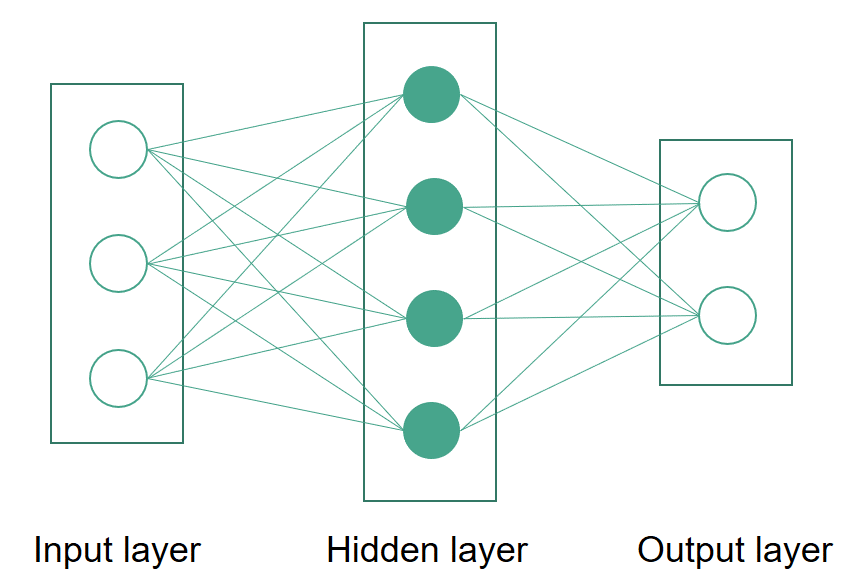
\includegraphics[width=0.7\textwidth]{bachproef/img/neuraalnetwerk.png}
\caption{Voorbeeld van een neuraal netwerk met 3 lagen}
\end{figure}

\vspace{1em}
De neuronen zijn verbonden met elkaar. In de figuur stellen de pijltjes de verbindingen voor, de verbindingen hebben elk een gewicht. Het gewicht geeft aan hoe essentieel de verbinding is. In het geval van dit onderzoek zal bijvoorbeeld het gebruikersdoel een groot gewicht krijgen omdat dit een belangrijke factor is bij het voorspellen. 

De neuronen bevatten ook een zogenaamde activatie functie. De werking hiervan wordt niet besproken omdat deze zeer complex is, maar eenvoudig gezegd standaardiseert de functie de uitvoer van de neuronen. 

\vspace{2em}
\begin{figure}[h!]
\centering
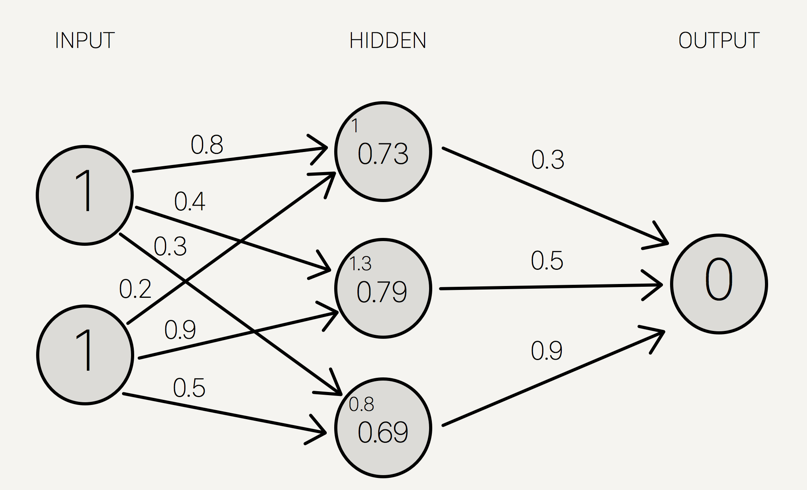
\includegraphics[width=0.7\textwidth]{bachproef/img/gewichten_netwerk.png}
\caption{Neuraal netwerk met gewichten}
\end{figure}

\newpage

\textbf{Trainen van het neuraal netwerk}

Om voorspellingen te kunnen doen is het trainen van een neuraal netwerk noodzakelijk. In dit onderzoek zullen de inzendingen van de vragenlijst dienen als trainingsdata. Er zal moeten duidelijk gemaakt worden aan de machine wat de invoervelden en wat de uitvoer is. Dit is makkelijk te doen in dit onderzoek omdat we gebruik maken van een CSV-bestand. We kunnen duidelijk aangeven dat bepaalde kolommen de invoer zijn en dat de overige kolom de uitvoer is.

In het begin van dit trainingsproces zal de computer soms een goed en soms een minder goede voorspelling maken. Dat is normaal, maar het is belangrijk om een kostfunctie te voorzien die berekent hoe fout de voorspelling nu is. Dit hebben we nodig om de voorspellingen beter te maken in de toekomst.

\textbf{De kostfunctie}


Het beste scenario is dat de kostfunctie gewoon 0 is, omdat dat wil zeggen dat de gemaakte voorspelling overeenstemt met de werkelijke uitkomst. Helaas is dit makkelijker gezegd dan gedaan. 

Het is mogelijk om willekeurige gewichten te zoeken zodat de kostfunctie minimaal is, maar de ze manier is alles behalve efficiënt. Daarom wordt er gebruik gemaakt van een techniek genaamd ‘Gradient Descent’. 

De Gradient Descent werkt volgens iteraties, per iteratie zal het logaritme de gewichten met een kleine waarde aanpassen. Na iedere iteratie wordt de kostfunctie berekend, zo kan er bepaald worden in welke richting de gewichten moeten aangepast worden om het minimum te vinden.

In geval van dit onderzoek wordt de berekening van de Gradient Descent automatisch gedaan.

\section{Deep Learning in de praktijk}

De antwoorden op de vragenlijst zal dus niet enkel gebruikt worden om de requirements van een applicatie te bepalen, maar de data zal ook gebruikt worden om Deep Learning toe te passen. Dit is het tweede grote deel van dit onderzoek.

\subsection{Gebruikte technologie}

Er zal gebruik gemaakt worden Python om de machine learning omgeving op te zetten. Om Python te kunnen coderen zal er gebruik gemaakt worden van PyCharm. PyCharm is een ontwikkelomgeving die speciaal gemaakt is voor het maken van Python applicaties. 
\newpage
De reden waarom er voor PyCharm is gekozen is omdat er veel documentatie te vinden is over deze omgeving. PyCharm biedt ook de mogelijkheid om externe code bibliotheken te gebruiken die we nodig hebben voor Deep Learning te kunnen toepassen.

Er bestaat veel voorgeprogrammeerde software om datasets te analyseren aan de hand van Deep Learning. Daar is bewust niet voor gekozen binnen dit onderzoek omdat het de bedoeling is dat er zelf code geschreven wordt om zo beter de werking te begrijpen.

\subsection{Gebruikte bibliotheken}

Het is quasi onmogelijk om alles volledig zelf te coderen, daarom worden er vele code bibliotheken of API’s aangeboden om voorgebakken methodes en functies te gebruiken in een zelfgeschreven applicatie. 

Als eerste wordt er gebruik gemaakt van Keras 2.0. Dit is een high-level API die eenvoudig en snel te gebruiken is. Keras biedt een framework aan om ‘deep learning’ neurale netwerken aan te maken met behulp van Python. 

Keras doet niet al het werk, de bibliotheek is enkel de ‘front-end’ laag die gebruik maakt van onderliggende lagen, in dit geval zijn dit andere bibliotheken. Keras is ontwikkeld door onderzoekers die de belangrijkste functionaliteiten in een bibliotheek hebben gebundeld. In dit onderzoek zal er gebruik gemaakt worden van Keras en onderliggend Tensorflow.
 
Dit biedt vele voordelen omdat enkel de Keras laag gebruikt zal worden om mee te coderen, terwijl Keras op zijn beurt gebruik maakt van Tensorflow achter de schermen. Daardoor kan er veel bereikt worden met een beperkt aantal lijnen code.

De onderliggende laag Google Tensorflow is een veel complexer algoritme, want dit is namelijk een low level API. Google translate maakt bijvoorbeeld ook gebruik van Tensorflow om betere vertalingen te kunnen voorspellen in de toekomst of om geen 2 keer dezelfde taalfout te maken. Deze complexiteit is niet nodig binnen het onderzoek, er zal enkel gebruik gemaakt worden van standaardmethodes. 

\subsection{Proof of concept: Deep Learning machine}

\textbf{Preprocess data}

Het gegenereerde CSV-bestand van onze vragenlijst is de input voor Deep Learning. De computer kan niet goed overweg met woorden, daarom moet de data omzet worden naar numerieke waarden. In dit onderzoek is gekozen om gebruik te maken van een ‘datascaler’ die alle waardes zal schalen tussen 0 en 1. Hiervoor gebruiken we ‘preprocess\_data.py’ deze code kan terug gevonden worden in de bijlage. Voorbeeld van deze uitvoer:
\newpage

\vspace{2em}
\begin{figure}[h!]
\centering
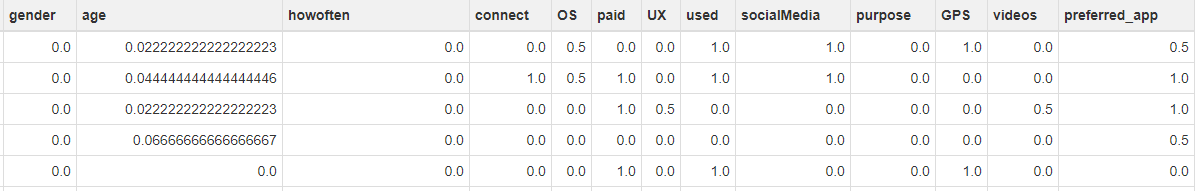
\includegraphics[width=1\textwidth]{bachproef/img/preprocess.png}
\caption{Preprocessing data}
\end{figure}

Alle woorden zijn omgezet naar een numerieke waarde waarmee bewerkingen kan maken. Merk op dat de computer voor gelijke woorden ook gelijke numerieke waardes neemt. 

\textbf{Data splitsen in trainingsdata en testdata}

De computer heeft behoefte aan 2 datasets, namelijk een dataset om zijn neuraal netwerk te trainen en de testdataset. De testdata heeft de computer nooit eerder gezien, deze data zal gebruikt worden om in een latere fase het foutratio van de voorspellingen te meten. Het is belangrijk dat de testdata nooit overeenkomt met de trainingsdata want dit kan een fout beeld geven over de trainingsvooruitgang.

\textbf{Creëren van een neuraal netwerk met Keras 2.0}

Zoals eerder uitgelegd in dit onderzoek, moet er een model gemaakt worden op voorwaarde dat een computer voorspellingen kan maken. Er is gekozen om gebruik te maken van 5 lagen: 1 inputlaag, 3 verborgen lagen en 1 uitvoerlaag. 

Het is belangrijk om de juiste dosering te vinden, anders kan dit leiden tot under- en overfitting. In het geval van underfitting is het logisch dat de voorspellingen niet correct zullen zijn omdat het model niet flexibel genoeg is, maar het model mag ook niet te flexibel zijn omdat dit dan tot overfitting zal leiden. In onderstaande figuur wordt under- en overfitting visueel voorgesteld: 

\vspace{2em}
\begin{figure}[h!]
\centering
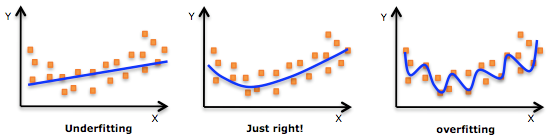
\includegraphics[width=1\textwidth]{bachproef/img/overfitting.png}
\caption{Visuele vergelijking van under - en overfitting}
\end{figure}

\newpage

\textbf{Model trainen en hergebruikbaar maken}

Als alle voorwaarden van hierboven voldaan zijn dan is de data klaar om getraind te worden. Eerst dient de kostfunctie gedefinieerd te worden, in dit onderzoek is er gekozen om met de kwadratische afwijking te werken. Daarna kunnen we effectief beginnen met het trainen van het neurale netwerk. 

De methode ‘fit’ zorgt hiervoor, er worden enkele parameters meegegeven: de invoer kolommen, de uitvoerkolommen en aantal herhalingen zijn hier de meest belangrijke. Merk ook op dat het belangrijk is dat de invoer en uitvoerkolommen gesplitst worden voor het trainingsproces!

Als er een parameter meegegeven wordt dan kan er ook een uitvoer gegenereerd worden van het trainingsproces, hieronder zijn enkele lijnen van deze uitvoer te vinden.

\begin{table}[h!]
\begin{center}
\begin{tabular}{ |p{6cm}|p{6cm}| }
 \hline
 \textbf{Herhaling}   &  \textbf{Kostenfunctie} \\
 \hline
Epoch 1/75 &  - loss: 0.1796  \\
 \hline
 Epoch 15/75 &  - loss: 0.0301  \\
 \hline
 Epoch 30/75 &  - loss: 0.0166  \\
 \hline
 Epoch 45/75 & - loss: 0.0176 \\
 \hline
 Epoch 60/75 & - loss: 0.0145 \\
 \hline
 Epocht 75/75 & - loss: 0.0145\\
 \hline
\end{tabular}
\end{center}
\caption{Uitvoer kostenfunctie bij Deep Learning}
\label{table:1}
\end{table}

In de tabel zijn een aantal herhalingen getoond van het proces, na iedere herhaling wordt de kosten functie berekend. Het is duidelijk zichtbaar dat de computer beter getraind is bij de laatste herhaling dan bij de eerste. Bij de eerste herhaling heeft de computer een foutratio van 17.96\% en bij de laatste slecht een foutratio van 1.45\%. 

Lager dan dit zal bijna onmogelijk zijn in het geval van dit onderzoek omdat we slechts maar een beperkt aantal lijnen trainingsdata hadden. Indien dit groter was geweest, dan kon het foutratio zeker nog omlaag.

Eens het model getraind is, kan de het model opgeslagen worden in een h5-bestand. Het bestand zal dus de structuur en gewichten bevatten om in de toekomst onze voorspellingen te doen. De reden dat dit in een h5-bestand opgeslagen wordt, is omdat dit een binair bestandstype is die ontworpen is om Python array data op te slaan. Er zijn ook nog andere varianten. 

\textbf{Training visualiseren met Tensorboard}

Een groot voordeel van Tensorflow is dat ze visualisatie ondersteunen. Het is mogelijk om de kostfunctie te visualiseren zoals in onderstaande afbeelding via een URL op een Localhost service:

\vspace{2em}
\begin{figure}[h!]
\centering
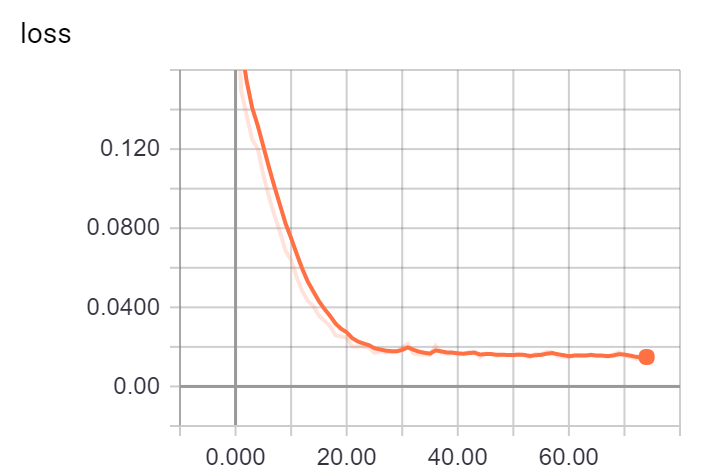
\includegraphics[width=0.7\textwidth]{bachproef/img/training_tensor.png}
\caption{Tensorboard trainingsproces}
\end{figure}

Op de Y-as zien we de kostenfunctie en op de X-as worden de iteraties afgebeeld. Ook visueel is het dus duidelijk dat de computer beter wordt naar mate het aantal iteraties. Op een gegeven moment blijft het wel gelijk. Dit komt, zoals er eerder is vermeld, door de beperkte trainingsdata.

Het is ook mogelijk om het denkpatroon van de computer te visualiseren met alle gewichten om aan de juiste uitvoer te komen. Hieronder staat een foto van het begin:

\begin{figure}[h!]
\centering
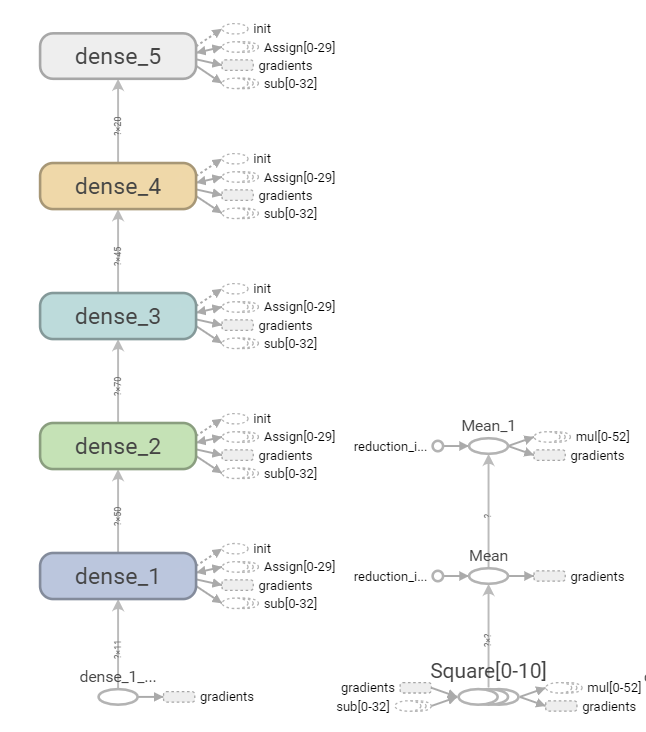
\includegraphics[width=0.5\textwidth]{bachproef/img/tensorboard.png}
\caption{Tensorboard trainingsproces}
\end{figure}
